% ~ 8-10 pages
\chapter{Decay Mode Classification of Hadronically Decaying $\tau$-Leptons}
\label{sec:decaymode}

In this chapter the sequence learning techniques developed for
tau-identification are applied to the problem of decay mode classification of
hadronic tau-lepton decays. In the following the decay modes containing one
charged hadron $h^\pm$ with one $h^\pm \pi^0$ or more than one neutral pion
$h^\pm \geq 2\pi^0$ as well as three charged hadrons without neutrals $3h^\pm$
or at least one neutral pion $3h^\pm \geq 1\pi^0$ shall be discriminated. The
hadron $h^\pm$ includes charged pions as well as kaons while decays over
intermediate $\text{K}^0$ are omitted. These five decay modes make up the
majority of hadronic tau-lepton decays (approx. \SI{92}{\percent}). Neural
networks naturally extend from binary to multi-class classification problems
making them well-suited for the discrimination of the hadronic decay modes.

At first a quick overview of the \emph{Tau Particle Flow}-Algorithm is given,
which is used to reconstruct neutral and charged decay products. Subsequently a
neural network is developed that uses the reconstructed decay products to
classify the decay mode into one of five categories. Finally the network is
extended by including additional information from conversion tracks, cluster
moments and shot information. In the following the notation established in
\cite{atlas:taurec:decaymodes} will be adopted.

\todo[inline]{Signature of the decay modes (Could be moved to
  \textit{Theoretical Background})}

\section{Tau Particle Flow}
\label{sec:tau_pflow}

The \emph{Tau Particle Flow}-algorithm is a specialised particle flow algorithm
for reconstruction of charged and neutral constituents in hadronic tau-lepton
decays with visible transverse momenta of up to \SI{100}{\giga\electronvolt}. It
aims to improve reconstruction of individual particles by optimally combining
the information in several subdetector-systems. The reconstructed objects,
called charged or neutral \emph{particle flow objects}~(PFOs), can be used to
classify the decay mode of hadronic tau-lepton decays and for improving the
energy resolution of the reconstructed hadronic tau decay by employing a decay
mode specific calibration. The following description of the algorithm is based
on \cite{atlas:taurec:decaymodes} including recent changes to the reconstruction
algorithms.

Charged PFOs are reconstructed from tracks classified as \emph{charged}
according to the track classification. The charge and transverse momentum of the
reconstructed PFO is determined from the measurement in the tracking system,
which has superior energy resolution for charged pions with
$p_\text{T} < \SI{100}{\giga\electronvolt}$ compared to a calorimeter-based
measurement \todo{Citation}. The $\pi^\pm$-mass hypothesis is used to calculate
the energy of the PFO. Charged hadrons initiate extensive hadronic showers
depositing most of their energy in the hadronic calorimeters (incl.\ EM3)
\todo{Motivation for this sentence?}.

Neutral pions often deposit their energy in a single cluster in the EM
calorimeter (Presampler, EM1/EM2) caused by two collimated photons from the
$\pi^0$ decay. Therefore neutral PFOs are reconstructed by clustering all cells
in the electromagnetic part of the calorimeter within the $\Delta R < 0.4$ cone
about the tau axis \todo{Check instead of core-region?}. If a cluster is in the
proximity of a charged PFO then the energy deposition of the charged hadron in
the EM calorimeter has to be separated from the neutral pion energy. The energy
$E_{h^\pm}^{\text{EM}}$ that needs to be subtracted to remove the contribution
of the charged hadron is estimated by
\begin{align*}
  E_{h^\pm}^{\text{EM}} = E_{h^\pm}^{\text{track}} - E_{h^\pm}^{\text{HAD}} \eqcomma
\end{align*}
where $E_{h^\pm}^{\text{track}}$ is the energy of the charged PFO measured in
the tracking system and $E_{h^\pm}^{\text{HAD}}$ the energy of the charged PFO
deposited in the hadronic part of the calorimeter. $E_{h^\pm}^{\text{HAD}}$ is
calculated by matching clustered energy deposits in the HCAL to the closest
track of a charged PFO. The contribution of the charged hadron in the EM
calorimeter~$E_{h^\pm}^{\text{EM}}$ is subtracted from the closest neutral PFO
cluster if the angular distance between cluster and extrapolated track is
smaller than $\Delta R < 0.04$. \todo{Zero mass hypothesis for neutrals?}
Neutral PFOs can often be reconstructed from an incomplete subtraction of the
charged hadron energy deposition in the EM calorimeter or by pile-up. For decay
mode classification it is necessary to identify the neutral pions in all
reconstructed neutral PFOs of the tau decay. The identification exploits the
difference in shower shape of hadronic showers initiated by charged hadrons and
compact showers from photons of the $\pi^0$ decay using multivariate methods.

The number of identified neutral pions can be used for a preliminary
classification of the decay mode. The following sections will be concerned with
combining reconstructed PFOs in neural networks to achieve better classification
power. Decay mode classification employing the \emph{Tau Particle
  Flow}-algorithm is optimised for operation in the low-momentum regime due to
the decreasing momentum resolution in the tracking system as well as the
additional boost of the tau decay products leading to merging of
$\pi^0$-clusters. Therefore this chapter focuses focus on the classification of
hadronic tau lepton decays with visible transverse
momenta~$p_\text{T} < \SI{100}{\giga\electronvolt}$.

\section{General Idea}
\todo{Better name for this part}
\label{sec:pfo_general}

The charged and neutral PFOs reconstructed with the \emph{Tau Particle
  Flow}-algorithm contain information about the daughter particles of the tau
decay and can be used for decay mode classification. Properties of charged and
neutral PFOs are combined in recurrent neural networks to perform multi-class
classification. Mainly kinematic information (e.g.\ transverse momentum, angular
deviation from the tau axis) is used to describe each PFO. Moreover the
$\pi^0$-likeness in form of the neutral pion identification BDT score is
included in the classification to be able to discriminate between neutral PFOs
originating from a $\pi^0$ and remnants of the subtraction.

\begin{figure}[htb]
  \centering
  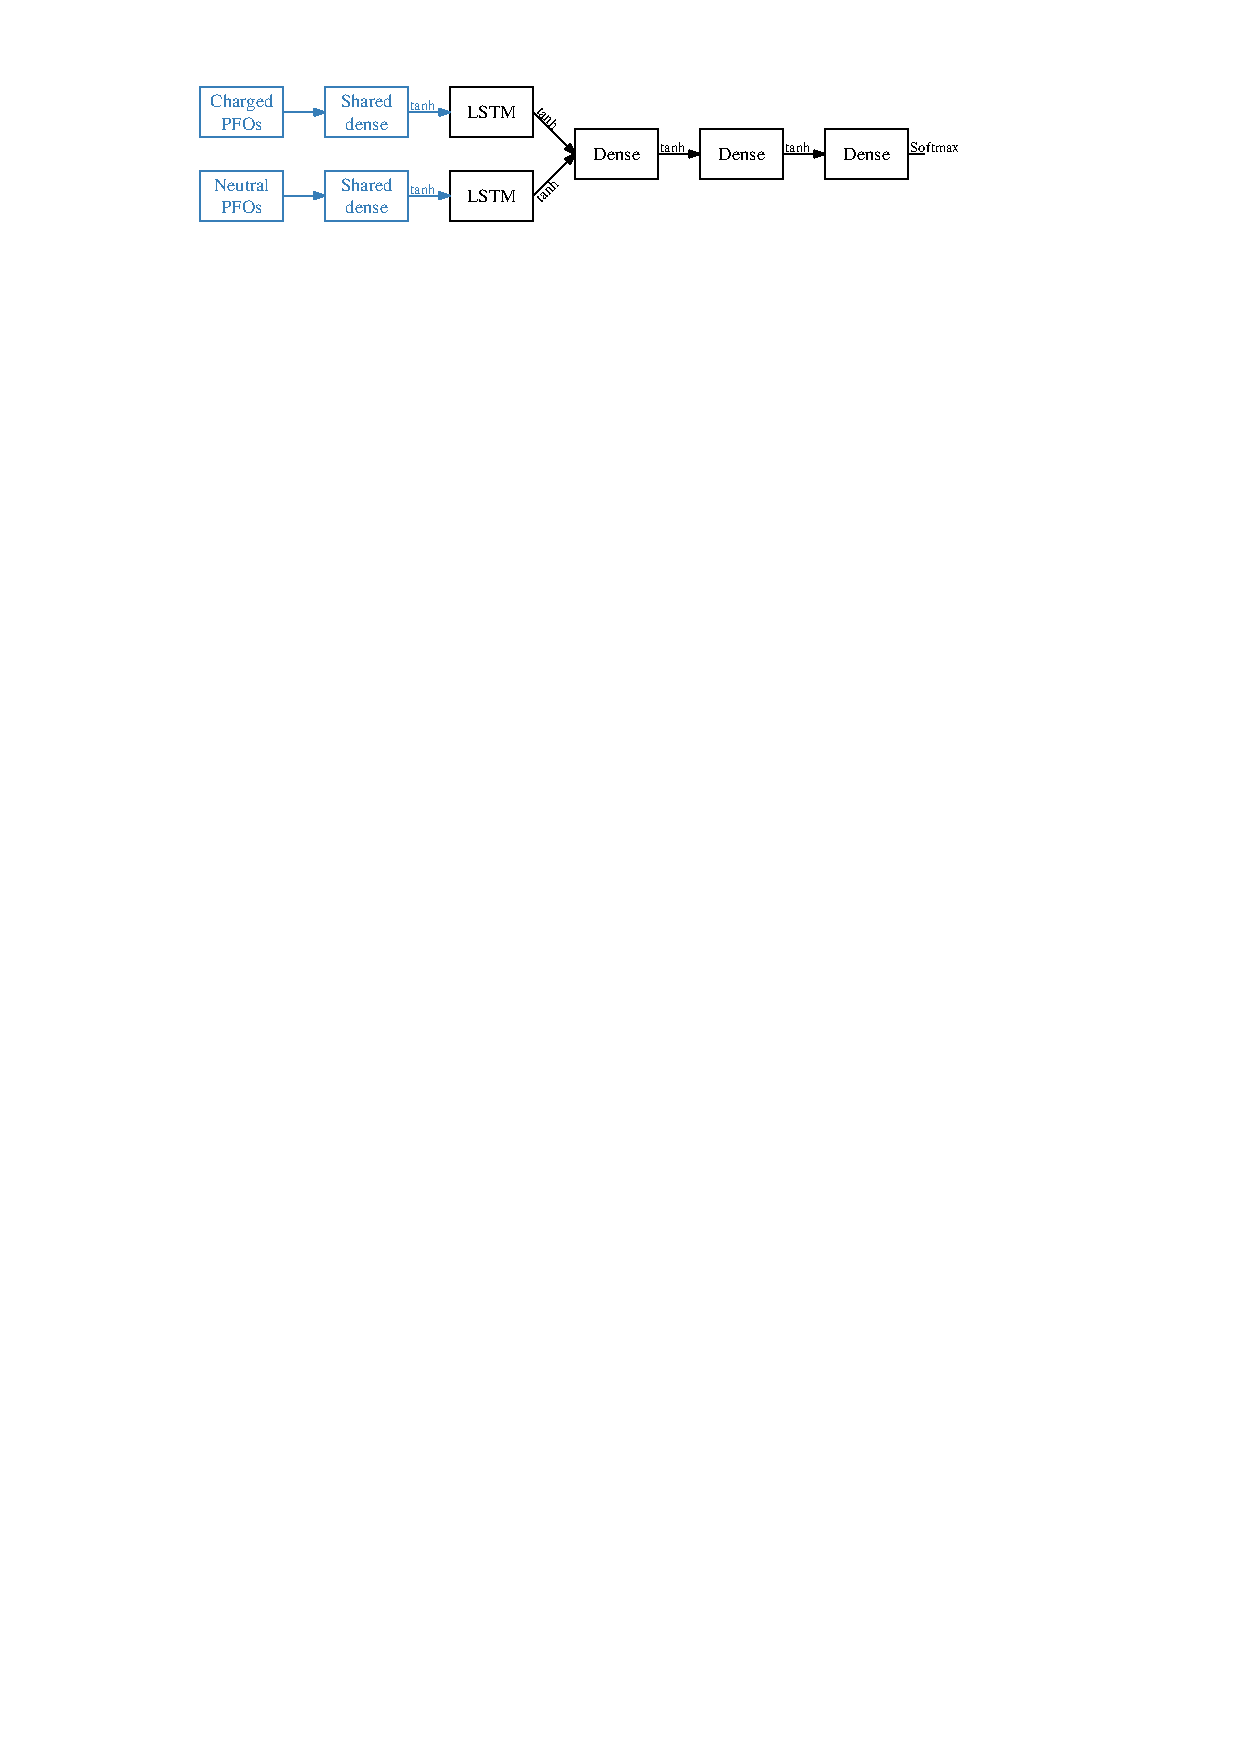
\includegraphics{./figures/decay_mode_classification/baseline_architecture.pdf}
  \caption{Architecture. Highlighted in blue are layers that operate on a sequence of inputs.}
  \label{fig:pfo_rnn_baseline_arch}
\end{figure}

The network architecture used for the decay mode classification is shown in
figure \ref{fig:pfo_rnn_baseline_arch} and is similar to the networks used for
tau-identification in the previous chapter. At the input layer the network is
split into two branches each accepting a number of charged and neutral PFOs
respectively. The shared dense layer\footnote{Applies the same transformation on
  every element of the input sequence} applies an affine transformation on the
input variables of each PFO. Afterwards the input sequences are fed into the
recurrent LSTM layer which subsequently return a single vector of activations.
The activations of both branches are then merged and passed through a network
containing three dense layers. The final dense layer has five units (the number
of decay modes to classify) which are activated by the Softmax activation
function, ensuring that the output activations sum to one.

\todo[inline]{Preselection (same as ID); Low momentum taus:
  $\SI{20}{\giga\electronvolt} < p_\text{T} < \SI{100}{\giga\electronvolt}$;
  Track requirement 1- or 3-prong; Truth decay mode}

\todo[inline]{During the classification the prongness of the decay mode is not
  constrained -- add. migrations are possible}

\section{Baseline}
\label{sec:pfo_baseline}

For training and evaluation of the model a sample containing the process
$\gamma^* \rightarrow \tau \tau \, \text{(hadr.)}$ is used (full sample
identifier in appendix~\ref{sec:app_mc16a_taus}). The baseline tau selection
given in section~\ref{sec:bdt_eventsim} is applied and the visible transverse
momentum~$p_\text{T}$ of the hadronic decay is required to be less than
\SI{100}{\giga\electronvolt} at reconstruction and generator-level. Moreover
only tau-leptons with the true decay mode being one of $h^\pm$, $h^\pm \pi^0$,
$h^\pm \geq 2\pi^0$, $3h^\pm$ or $3h^\pm \geq 1\pi^0$ and omitting decay chains
containing intermediate $\text{K}^0$.

The discrimination of the decay modes utilises kinematic quantities of the
reconstructed tau decay as well as the charged and neutral particle flow
objects:
\begin{description}
\item[Kinematic quantities of the tau decay:] The visible transverse momentum
  $p_\text{T}^\tau$ and the direction $(\varphi_\tau, \eta_\tau)$ of the
  reconstructed tau-axis. The momentum is calibrated at LC-scale
  without applying a tau-specific energy calibration.

\item[Kinematic quantities of charged and neutral PFOs:] The reconstructed
  transverse momentum $p_\text{T}^\text{PFO}$ and the signed angular distances
  to the reconstructed tau decay in transverse\footnote{The definition is
    analogous to the longitudinal case but also accounting for the periodicity
    in $\varphi$.}~$\Delta\varphi$ and longitudinal
  direction~$\Delta\eta \coloneqq \eta_\text{PFO} - \eta_\tau$. The PFO
  directions are given relative to the tau-axis to ensure that coordinates are
  comparable for different tau candidates.
\end{description}
Furthermore the variable set used for the neutral PFOs is extended using:
\begin{description}
\item[$\pi^0$ identification score $S_\text{BDT}^{\pi^0}$:] BDT-based
  discriminant combining cluster information in the electromagnetic part of the
  calorimeter to identify neutral PFOs originating from the $\pi^0$ decay.

\item[Number of shots $N_\text{shots}$:] Number of shots (cmp.\
  section~\ref{sec:shot_reco}) associated with a neutral PFO cluster. Shots are
  associated with a cluster if it contains the seed cell of the shot and the
  cluster fulfils $E_\text{T} > \SI{500}{\mega\electronvolt}$ and is within
  $\Delta R < 0.4$ to the tau axis. In cases where the cell is shared between
  multiple clusters, it is associated to the cluster to which the seed cell
  contributes with the largest weight.

  The fine segmentation of the strip layer of the EM calorimeter is used to
  count local energy maxima created by individual photons and allow to recover
  the correct number of neutrals in cases where the energy depositions of two
  neutral pions are reconstructed as a single cluster in the calorimeter.
\end{description}
\todo[inline]{Give reasons for this variable selection. \SI{1.5}{\percent}}

\todo[inline]{Preprocessing:} The transverse momenta of the reconstructed tau as
well as the PFOs are log-transformed and subsequently standardised (by
subtracting the mean and dividing by the standard deviation of the transformed
variable). The remaining kinematic variables are transformed to fall into the
the $[-1, 1]$ range. For the neutral PFO specific variables
$S_\text{BDT}^{\pi^0}$ and $N_\text{shots}$ no preprocessing is needed.

Charged and neutral PFOs are passed in ascending transverse momentum ordering to
the shared dense layers with 24 units each. The intermediate representation of
the input sequence is then passed into the LSTM layers each with 24 units and
hard sigmoid recurrent activation. The recurrent layers return a single element
containing 24 scalar values which are subsequently merged and passed through
three dense layers with 48, 32 and 5 units respectively. The outputs of the
different layers are activated using the $\tanh$ activation function with the
exception of the last dense layer, which uses \emph{Softmax} activation.

For each reconstructed tau decay the model returns one probability for each of
the five decay modes. The reconstructed decay mode is then given as the mode
with the highest probability according to the model. A different scheme for
determining the decay mode would be to require the largest mode probability to
exceed the second largest by a predefined margin. This would increase the purity
of the reconstructed modes at the expense of reducing the reconstruction
efficiency (should be evaluated on analysis-level).

In contrast to the decay mode classification algorithm currently in use at the
ATLAS experiment, no discrimination of 1- and 3-prong modes according to the
number of tracks that are classified as \emph{charged} is made. However each
charged PFO is associated with a \emph{charged} track such that the number of
tracks is indirectly available to the network. The network is not strictly
required to use this information allowing migrations of reconstructed 1-track
(3-track) hadronic tau decays to 3-prong (1-prong) modes. If this behaviour is
not desired then the decay mode can be classified as the mode with the highest
probability that is still compatible with the number of reconstructed tracks.

Reconstructed hadronic tau decays contain neutral PFOs that are not originating
from neutral pions but from other sources. Moreover it is not known how well
these PFOs are modelled in the simulation that is used to train and evaluate the
models. Therefore the neutral PFOs used in the RNN are required to pass a
$p_\text{T}$-threshold. Table \ref{tab:neut_ptcut} summarises the diagonal
efficiency of the classification for four different thresholds \todo{Requires
  retraining of the model!}.
\begin{table}[htb]
  \centering
  \begin{tabular}{SS[table-format=2.2(2)]}%,table-space-text-post = \si{\meter}]}
  \toprule
  {$p_\text{T}$-cut / \si{\giga\electronvolt}} & {Diagonal efficiency / \si{\percent}} \\
  \midrule
  {--} & 78.43 \pm 0.06 \\
  1.0 & 78.09 \pm 0.08 \\
  1.5 & 77.95 \pm 0.04 \\
  2.0 & 77.88 \pm 0.06 \\
  2.5 & 77.54 \pm 0.04 \\
  \bottomrule
\end{tabular}

%%% Local Variables:
%%% mode: latex
%%% TeX-master: "../mythesis"
%%% End:

  \caption{Impact of a neutral $p_\text{T}$-cut on the diagonal
    efficiency.}
  \todo[inline]{Motivate \SI{1.5}{\giga\electronvolt} cut.}
  \label{tab:neut_ptcut}
\end{table}
It is observed that the overall classification performance does not degrade when
no $p_\text{T}$-cut is applied, indicating that the network is able to (since
$p_\text{T}^\text{PFO}$ is an input). Moreover the accuracy does not decrease
drastically \todo{better word?} when the threshold is increased such that a
threshold can be applied if it turns out that low momentum PFOs show significant
mismodelling. For further studies the \SI{1.5}{\giga\electronvolt} threshold is
used.

\todo[inline]{Explain migration and composition matrices. Explain that the
  trainings are not 'stable' in the sense that classification power can be
  redistributed across different modes i.e.\ a decrease in one mode can be
  compensated by improvements in another.}

\begin{figure}[htb]
  \begin{subfigure}[t]{0.48\textwidth}
    \centering
    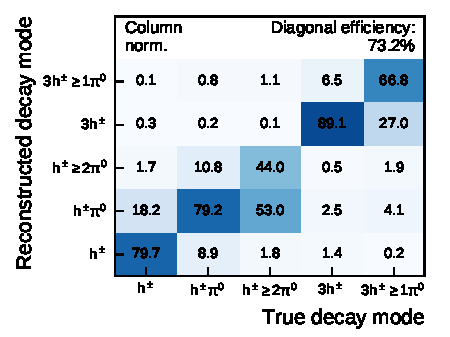
\includegraphics{./figures/decay_mode_classification/mig_mat_pantau.pdf}
    \subcaption{ATLAS default algorithm: \emph{PanTau}}
  \end{subfigure}\hfill
  \begin{subfigure}[t]{0.48\textwidth}
    \centering
    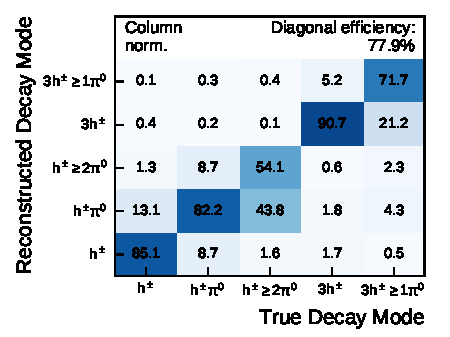
\includegraphics{./figures/decay_mode_classification/mig_mat_baseline_ptcut_1_5.pdf}
    \subcaption{PFO-RNN with neutral $p_{\text{T}}$-cut of
      \SI{1.5}{\giga\electronvolt}}
  \end{subfigure}
  \caption{Migration matrices with normalised columns showing the migration of
    the true decay modes to the reconstructed modes. }
  \todo[inline]{After reconstruction in
    $\gamma^* \rightarrow \tau \tau \, \text{hadr.}$ and omitting decays
    containing neutral kaons.}
  \label{fig:migmat}
\end{figure}


\begin{figure}[htb]
  \begin{subfigure}[t]{0.48\textwidth}
    \centering
    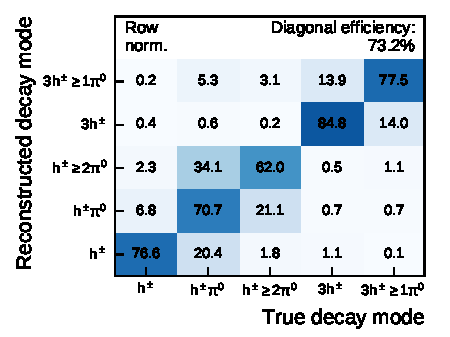
\includegraphics{./figures/decay_mode_classification/comp_mat_pantau.pdf}
    \subcaption{ATLAS default algorithm: \emph{PanTau}}
  \end{subfigure}\hfill
  \begin{subfigure}[t]{0.48\textwidth}
    \centering
    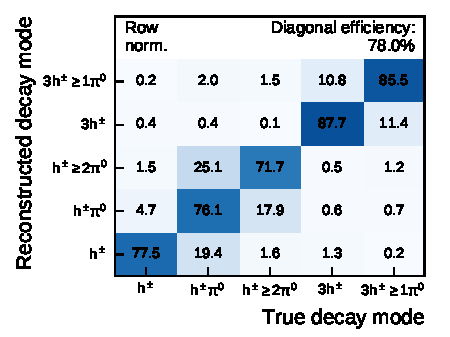
\includegraphics{./figures/decay_mode_classification/comp_mat_baseline_ptcut_1_5.pdf}
    \subcaption{PFO-RNN with neutral $p_{\text{T}}$-cut of
      \SI{1.5}{\giga\electronvolt}}
  \end{subfigure}
  \caption{Composition matrices with normalised rows showing the migration of
    the true decay modes to the reconstructed modes.}
  \label{fig:migmat}
  \todo[inline]{Check whether the 'diagonal efficiency' is correct for
    composition matrices.}
\end{figure}


\begin{figure}[ht]
  \begin{subfigure}[t]{0.48\textwidth}
    \centering
    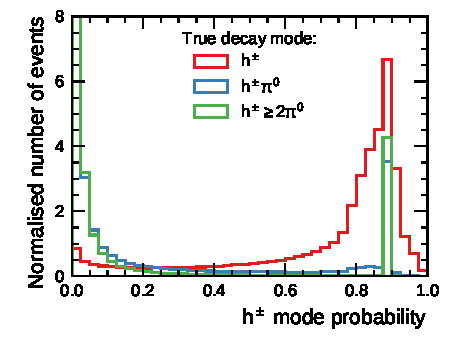
\includegraphics{./figures/decay_mode_classification/mode_proba_baseline_ptcut_1_5_only_1p/proba_1p0n.pdf}
    \subcaption{In most cases the probabilities for modes containing neutral
      pions to be classified as the $h^\pm$ mode are small. However in cases
      where no neutral PFO is reconstructed the probabilities can be large
      \SI{90}{\percent}.}
  \end{subfigure}\hfill
  \begin{subfigure}[t]{0.48\textwidth}
    \centering
    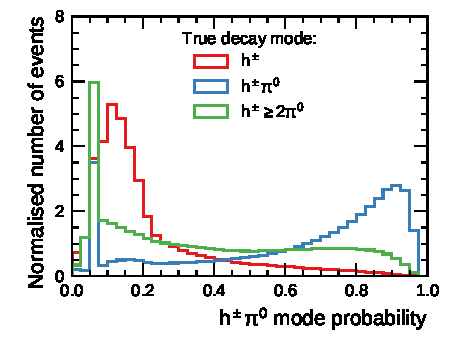
\includegraphics{./figures/decay_mode_classification/mode_proba_baseline_ptcut_1_5_only_1p/proba_1p1n.pdf}
    \subcaption{The discrimination of modes with one neutral and more than one
      neutral pion is difficult. In cases of no reconstructed neutral pions the
      probabilities can be small ($\approx \SI{5}{\percent}$)}
  \end{subfigure}
  \caption{Mode probabilities for the $h^\pm$ and $h^\pm \pi^0$ modes. While
    each tau candidate is assigned a probability for all five decay modes the
    probabilities for the 3-prong modes have been omitted.}
  \label{fig:mode_proba_ptcut}
\end{figure}

\section{Additional Information}

\begin{description}
\item[Conversion tracks] Often photons from the $\pi^0$ decay convert into
  electron-positron pairs in the material of the inner detector. Conversions can
  therefore \todo{Why? Electrons bent out of cone? Neutral PFOs fail $\pi^0$-ID?
    Will the electrons be reconstructed in neutral PFOs?} lead to an
  underestimation of the number of neutral pions. The inclusion of conversion
  tracks in the classification aims to reduce migrations to decay modes with
  fewer neutrals.

\item[Shots] Due to the boosted topology of tau decays in ATLAS (especially at
  high-$p_\text{T}$) neutral pion clusters can merge with the charged or another
  neutral pion leading to a reduction in the reconstructed number of neutrals.
  Information on nearby shots \todo{NHitsInEM1 is already in the neut.\ PFOs}
  can further improve classification.

\item[Add. cluster moments] Further improvements in classifying merged clusters
  can be achieved by using shower shape information similar to what is used for
  the $\pi^0$ identification.
\end{description}

\begin{description}
\item[Width $\langle R^2 \rangle$]
\item[$\eta$ width in EM1 $\langle (\eta - \eta_\text{cluster})^2\rangle$]
\item[Number of positive cells in EM1 $N_\text{EM1}^\text{pos}$]
\item[Core energy fraction $f_\text{core}$] Fraction of the total cluster energy
  contained in the highest energy cells in Presampler, EM1 and EM2.
\item[Energy fraction in EM2 $f_\text{EM2}$]
\end{description}
Longitudinal moments were not found to lead to an increase performance.


Neutral PFOs (Charged PFOs + whats listed here):
\begin{itemize}
\item $f_\text{core}$: \texttt{ENG\_FRAC\_CORE} Fraction of energy in the three
  hottest cells in each sampling \todo{Check}
\item $f_\text{EM2} = E_\text{EM2} / E$: Energy fraction in EM2 \todo{Why not
    EM1? -- Energy fraction is highly anti-correlated with EM1 therefore only
    one is chosen.}
\end{itemize}

\begin{table}[htb]
  \centering
  \begin{tabular}{p{5cm}S[table-format=1.4(4)]S[table-format=2.2(2)]S[table-format=1.2(2)]}
  \toprule
  {Experiment} & {Loss} & {Diag.\ eff.\ / \si{\percent}} & {Diag.\ eff.\ gain (abs.) / \si{\percent}} \\
  \midrule
  Conversion tracks & 0.5186 +- 0.0013 & 79.40 +- 0.07 & 1.45 +- 0.08 \\
  Conversion tracks (extrapol.) & 0.5224 +- 0.0012 & 79.23 +- 0.06 & 1.28 +- 0.07 \\
  Shots & 0.5239 +- 0.0011 & 79.52 +- 0.06 &  1.57 +- 0.07 \\
  Neut.\ PFO cluster properties & 0.5310 +- 0.0010 & 79.07 +- 0.06 & 1.12 +- 0.07 \\
  Hadronic PFOs & 0.5433 +- 0.0007 & 78.30 +- 0.04 & 0.35 +- 0.06 \\
  Fraction of subtracted $p_\text{T}$ & 0.5466 +- 0.0005 & 78.26 +- 0.03 & 0.31 +- 0.05 \\
  $\pi^0$-BDT ordering & 0.5511 +- 0.0013 & 78.01 +- 0.07 & 0.06 +-0.08 \\
  \bottomrule
\end{tabular}

%%% Local Variables:
%%% mode: latex
%%% TeX-master: "../mythesis"
%%% End:

  \caption{Additional experiments}
  \label{tab:pfo_add_experiments}
\end{table}

\begin{align*}
  f_\text{sub} = \frac{p_{\text{T}}^{\text{cluster}} - p_{\text{T}}^{\text{PFO}}}{p_{\text{T}}^{\text{PFO}}}
\end{align*}

\todo[inline]{Try out bidirectional LSTMs and stacked ones (still not
  overfitting).Technically would allow multiple outputs: Could do Pi0 Cluster-ID
  internally. What else has been tested?}

\section{Combining Everything}

\begin{figure}[!ht]
  \begin{subfigure}{0.48\textwidth}
    \centering
    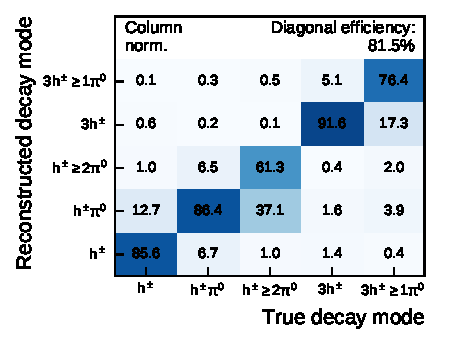
\includegraphics{./figures/decay_mode_classification/combined_sub_e_moments_shots_conv_ptcut_1_5/mig_mat.pdf}
    \subcaption{Migration matrix}
  \end{subfigure}\hfill
  \begin{subfigure}{0.48\textwidth}
    \centering
    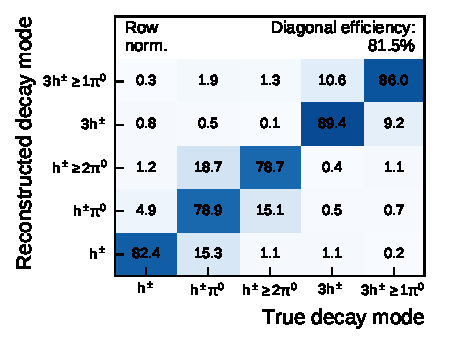
\includegraphics{./figures/decay_mode_classification/combined_sub_e_moments_shots_conv_ptcut_1_5/comp_mat.pdf}
    \subcaption{Composition matrix}
  \end{subfigure}
  \caption{Combined}
  \label{fig:decay_mode_combined}
\end{figure}

\begin{figure}[!ht]
  \begin{subfigure}{0.48\textwidth}
    \centering
    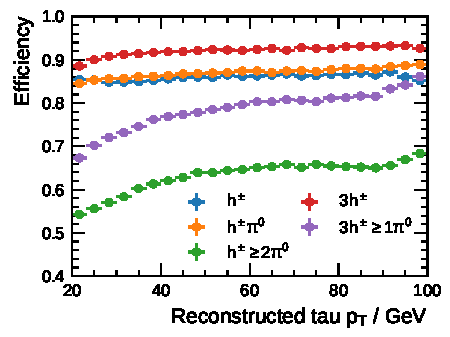
\includegraphics{./figures/decay_mode_classification/combined_sub_e_moments_shots_conv_ptcut_1_5/efficiency_profile.pdf}
    \subcaption{Efficiency profile}
  \end{subfigure}\hfill
  \begin{subfigure}{0.48\textwidth}
    \centering
    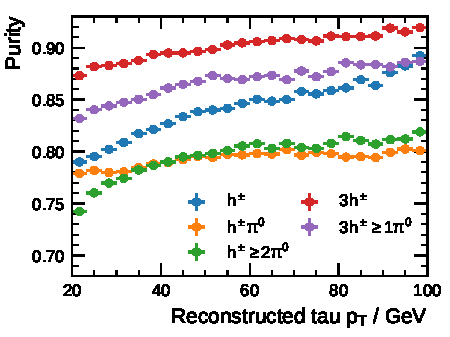
\includegraphics{./figures/decay_mode_classification/combined_sub_e_moments_shots_conv_ptcut_1_5/purity_profile.pdf}
    \subcaption{Purity profile}
  \end{subfigure}
  \caption{$p_\text{T}$-dependence of mode efficiency and purity}
  \label{fig:mode_efficiency_purity}
\end{figure}

\todo[inline]{Class probabilities (showing the non-existent peak). Improvements
  for Higgs CP measurement in
  $H \rightarrow \tau\tau \rightarrow \rho \rho 2\nu$. Performance when applying
  medium tau identification. Fluid classification -- a single PFO is not
  'causing' a particular classification result -- could use heuristic methods to
  reconstruct neutral pions after classification. Unleash on data without upper
  $p_\text{T}$ limit.}

\begin{table}[htb]
  \centering
  \begin{tabular}{
  l
  S[table-format=2.2(2)]
  S[table-format=2.1(2)]
  S[table-format=2.1, round-mode=places, round-precision=1]
  S[table-format=2.1, round-mode=places, round-precision=1]
  }
  \toprule
  {Mode} & {$\mathcal{B}$ / \si{\percent}} & {$f_\text{BR}$ / \si{\percent}} & {$f_\text{reco}$ / \si{\percent}} & { $f_\text{reco+ID}$ / \si{\percent}} \\
  \midrule
  $h^\pm$ & 11.51 +- 0.05 & 18.3 +- 0.1 & 17.552988 & 21.365416 \\
  $h^\pm \pi^0$ & 25.93 +- 0.09 & 41.3 +- 0.2 & 41.854581 & 44.779216 \\
  $h^\pm \geq 2 \pi^0$ & 10.81 +- 0.09 & 17.2 +- 0.2 & 18.663134 & 15.775690 \\
  $3 h^\pm$ & 9.43 +- 0.05 & 15.1 +- 0.1 & 14.200414 & 13.315444 \\
  $3 h^\pm \geq 1 \pi^0$ & 5.09 +- 0.05 & 8.1 +- 0.1 & 7.728881 & 4.764232 \\
  \bottomrule
\end{tabular}

%%% Local Variables:
%%% mode: latex
%%% TeX-master: "../mythesis"
%%% End:

  \caption{Mode reconstruction efficiencies. $h^\pm$ can be pion or kaon.
    Intermediate decays via neutral kaons are excluded. Branching fraction
    $\mathcal{B}$; Mode fractions of reconstructed taus passing preselection
    $f_\text{reco}$; Mode fraction of taus also passing medium tau id.}
  \todo[inline]{Do the fractions make sense? Make comparable to branching
    ratio?}
  \label{tab:mode_reco_eff}
\end{table}

\begin{figure}[!ht]
  \begin{subfigure}{0.48\textwidth}
    \centering
    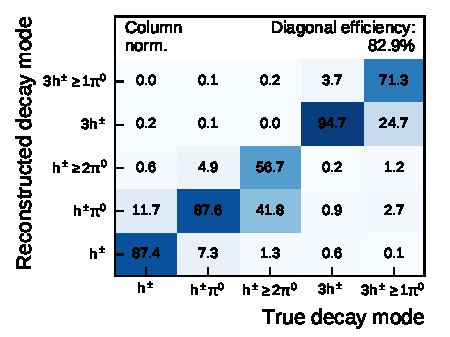
\includegraphics{./figures/decay_mode_classification/combined_sub_e_moments_shots_conv_ptcut_1_5/mig_mat_med_id.pdf}
    \subcaption{Migration matrix}
  \end{subfigure}\hfill
  \begin{subfigure}{0.48\textwidth}
    \centering
    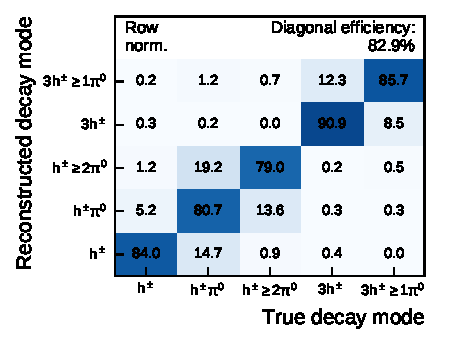
\includegraphics{./figures/decay_mode_classification/combined_sub_e_moments_shots_conv_ptcut_1_5/comp_mat_med_id.pdf}
    \subcaption{Composition matrix}
  \end{subfigure}
  \caption{Combined with medium tau id}
  \label{fig:decay_mode_combined_med_id}
\end{figure}

\clearpage
\subsection{High-$p_\text{T}$ performance}
\begin{figure}[htb]
  \begin{subfigure}{0.48\textwidth}
    \centering
    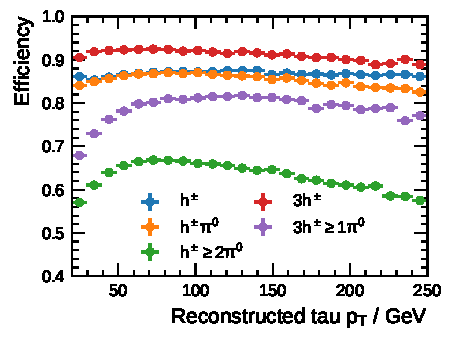
\includegraphics{./figures/decay_mode_classification/highpt/efficiency_profile.pdf}
    \subcaption{Efficiency profile}
  \end{subfigure}\hfill
  \begin{subfigure}{0.48\textwidth}
    \centering
    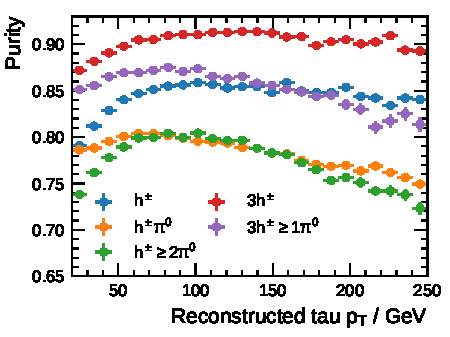
\includegraphics{./figures/decay_mode_classification/highpt/purity_profile.pdf}
    \subcaption{Purity profile}
  \end{subfigure}
  \caption{$p_\text{T}$-dependence of mode efficiency and purity}
  \label{fig:mode_efficiency_purity_highpt}
\end{figure}

\begin{figure}[htb]
  \begin{subfigure}{0.48\textwidth}
    \centering
    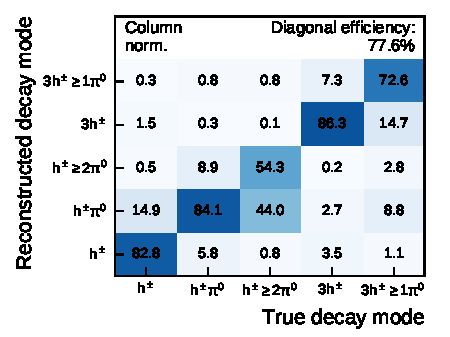
\includegraphics{./figures/decay_mode_classification/highpt/mig_mat_pt_geq_100.pdf}
    \subcaption{Migration matrix. $p_\text{T} > \SI{100}{\giga\electronvolt}$}
  \end{subfigure}\hfill
  \begin{subfigure}{0.48\textwidth}
    \centering
    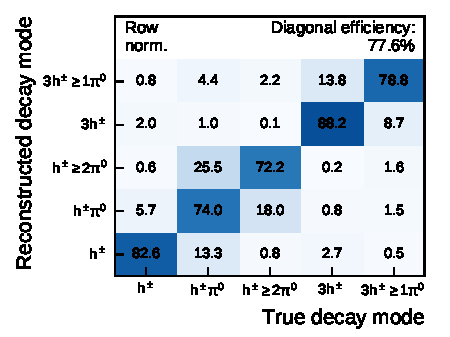
\includegraphics{./figures/decay_mode_classification/highpt/comp_mat_geq_100.pdf}
    \subcaption{Composition matrix. $p_\text{T} > \SI{100}{\giga\electronvolt}$}
  \end{subfigure}
  \caption{highpt}
  \label{fig:highpt_matrices}
\end{figure}


%%% Local Variables:
%%% mode: latex
%%% TeX-master: "mythesis"
%%% End:
